% Tikz File 'mytikz.tex'
\documentclass{standalone}
\usepackage{pgfplots}
\usepackage{tikz}

\usetikzlibrary{quotes,angles}

%\usetikzlibrary{...}
\begin{document}
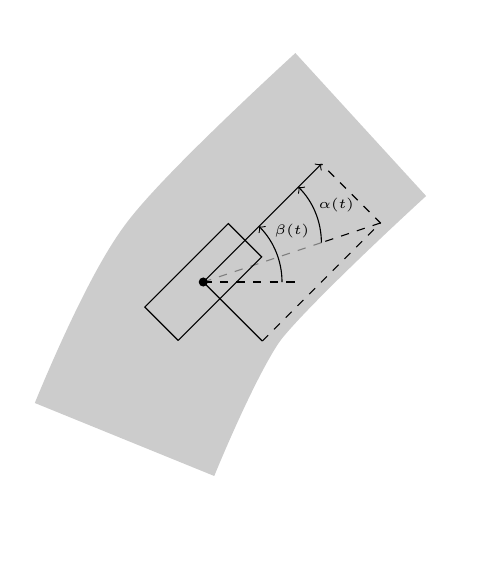
\begin{tikzpicture}
% course
  \draw [gray!40, line width = 70pt] plot [smooth] coordinates { (-1,-2) (0,0) (2,2)};
  
  \draw[->]
    (0.75,-0.75) coordinate 
    -> (0,0) coordinate 
    -> (1.5,1.5) coordinate;
  \draw[dashed]
   (0.75,-0.75) -- (2.25, 0.75) --(1.5,1.5);
   \draw[dashed]
   (2.25, 0.75) -- (1.5,0.5);
   \draw[dashed, gray!100]
   (1.5,0.5) -- (0,0);
   
   
  \draw[dashed]
  (0, 0) -- (1.2, 0);

% car
  \draw [rotate around = {45:(0,0)}]   (-0.75, -0.3) -- (0.75, -0.3) -- (0.75, 0.3) -- (-0.75, 0.3) -- (-0.75, -0.3);

% middle of the car
   \draw[fill] (0,0) circle [radius=0.05];
   
% angels

   \draw[->] (1,0) arc(0:45:1);
   \node[] at (30:1.3) {\tiny $\beta(t)$};
   \draw[->] (1.5,0.5) arc(0:45:1);
   \node[] at (30:1.95) {\tiny $\alpha(t)$};
   
   
   
\end{tikzpicture}
\end{document}